Clase: 30/08/2022

\begin{teorema}[Green]
    Sea $\gamma$ una curva cerrada, simple, orientada positivamente y suave por tramos en la región $D$ del plano acotada por $\gamma$. Si $P(x,y)$ y $Q(x,y)$ tienen derivadas continuas sobre $D$, entonces: 
    $$\int_\gamma P(x,y)dx+Q(x,y)dy=\iint_D\left(\frac{\partial Q}{\partial x}-\frac{\partial P}{\partial y}\right)dxdy$$
\end{teorema}

\begin{teorema}[Curva de Jordan]
    Una curva cerrada y simple secciona el plano $\mathbb{R}^2$ en dos subconjuntos conexos, uno de ellos acotado. 
    \begin{dem}
        Sea $f=u+iv$, una función analítica sobre y en el interior de $\gamma\implies \int_\gamma f = \int_\gamma (u+iv)(dx+idy)=\int_\gamma[(udx-vdy)+i(udy+vdx)]=\int_\gamma [udx-vdy]+i\int_\gamma[vdx +udy]=\iint_D\left[-\frac{\partial v}{\partial x}-\frac{\partial u}{\partial y}\right]dxdy +i\iint_D\left[\frac{\partial u}{\partial x}-\frac{\partial v}{\partial y}\right]dxdy$. Ambas integrales se hacen 0 por Cauchy-Riemman. 
    \end{dem}
\end{teorema}

\begin{teorema}[de Deformación]
    Sea $f$ analítica sobre una región $A$ y sea $\gamma$ una curva cerrada y simple sobre $A$. Suponga que $\gamma$ es homotópica a otra curva $\tilde{\gamma}$ sin salir de $A$. Entonces, 
    $$\int_\gamma f = \int_{\tilde{\gamma}}f$$ 
    \begin{figure}[H]
        \centering
        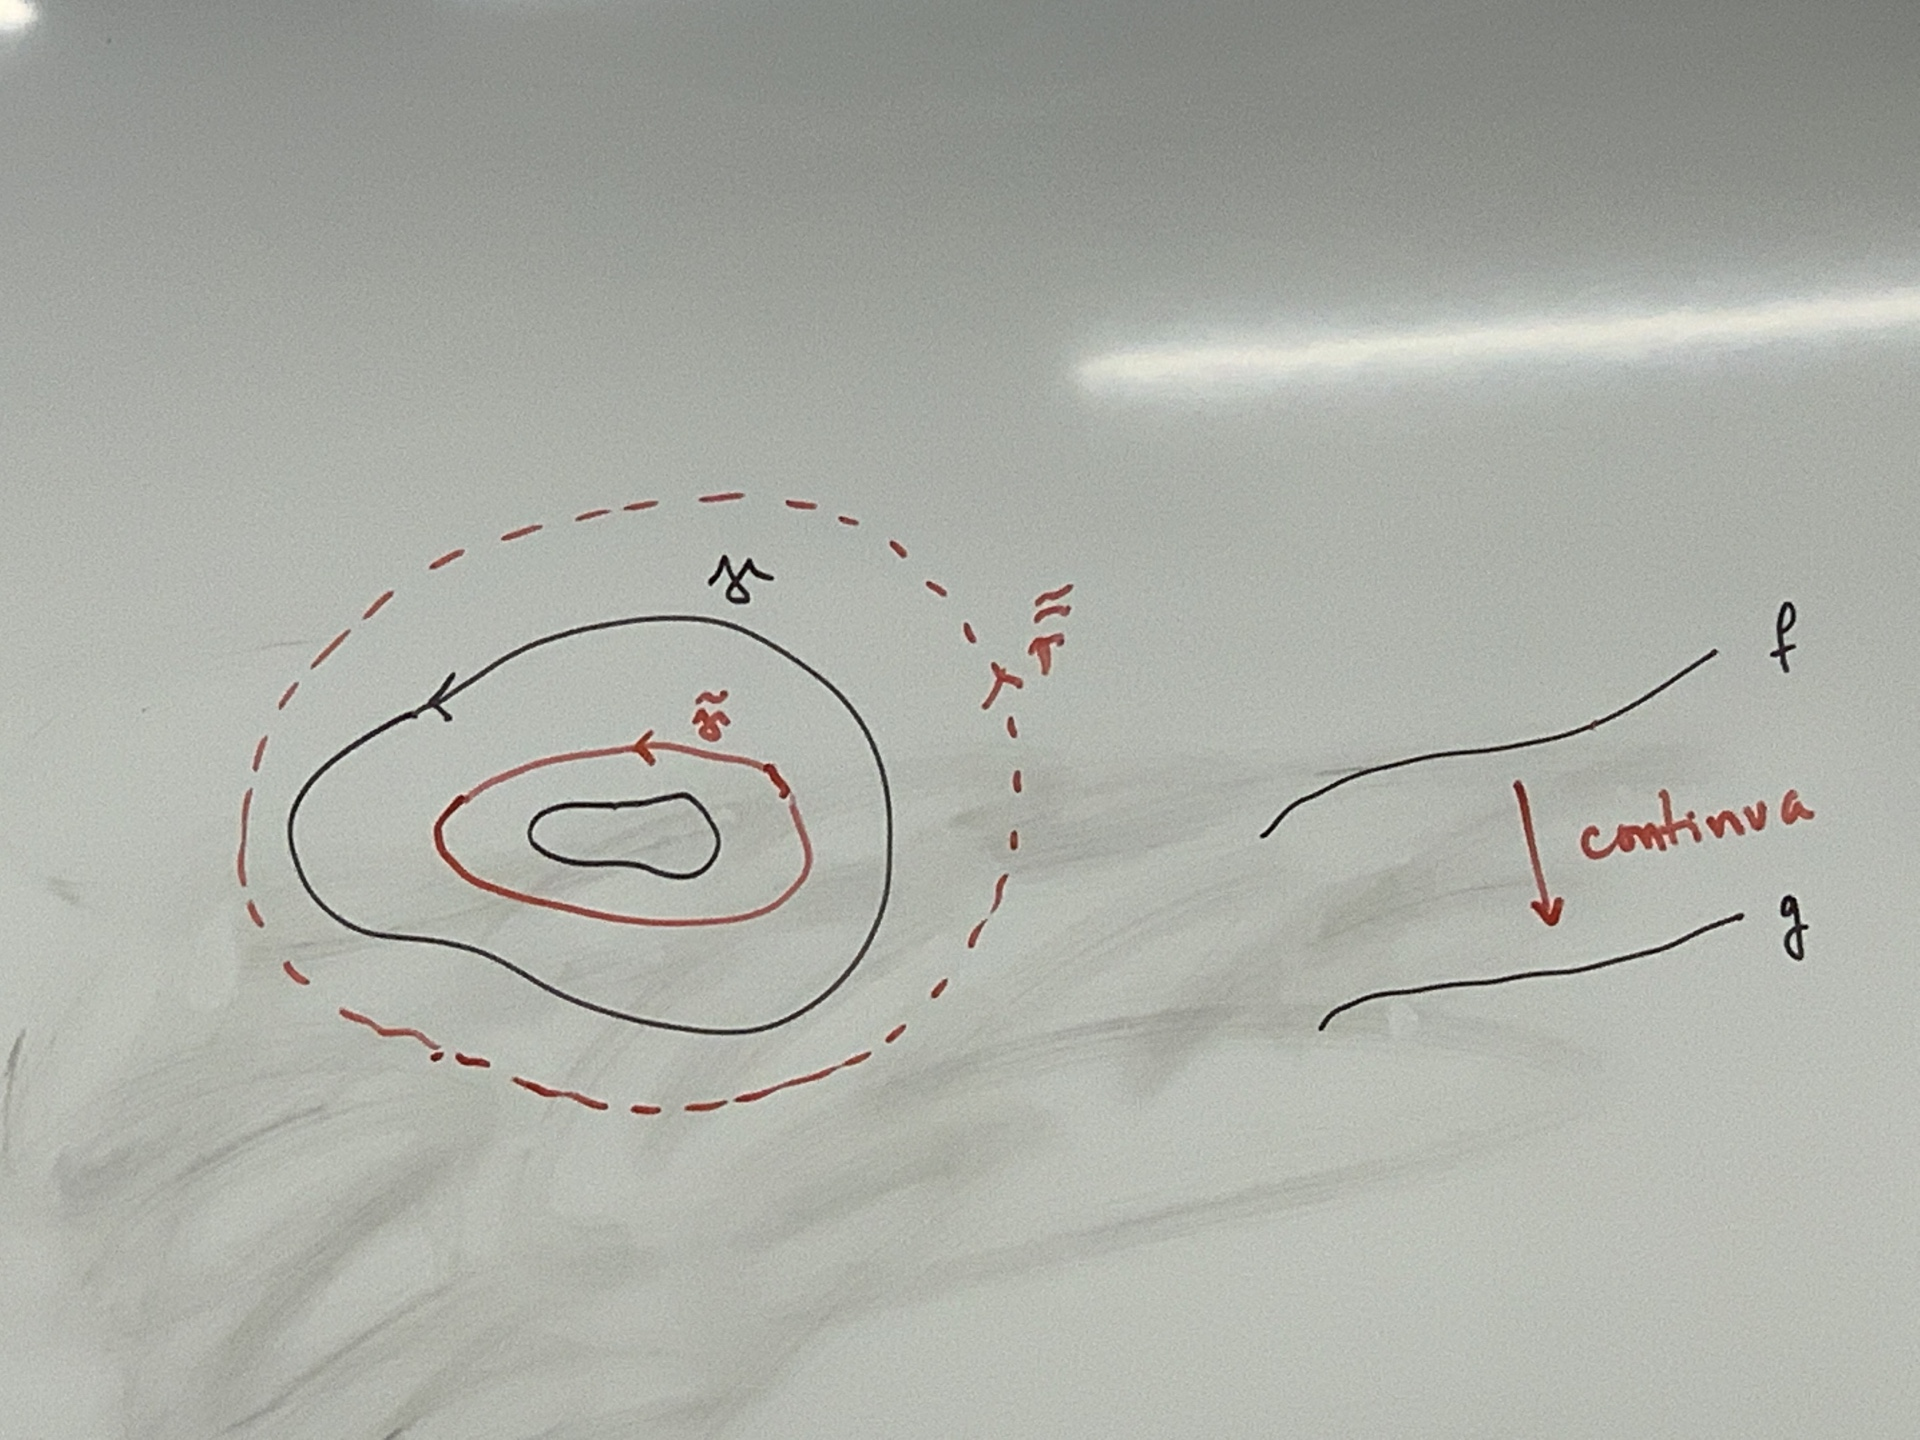
\includegraphics[scale=0.1]{imagenes/11.1.jpeg}
    \end{figure}
    \begin{figure}[H]
        \centering
        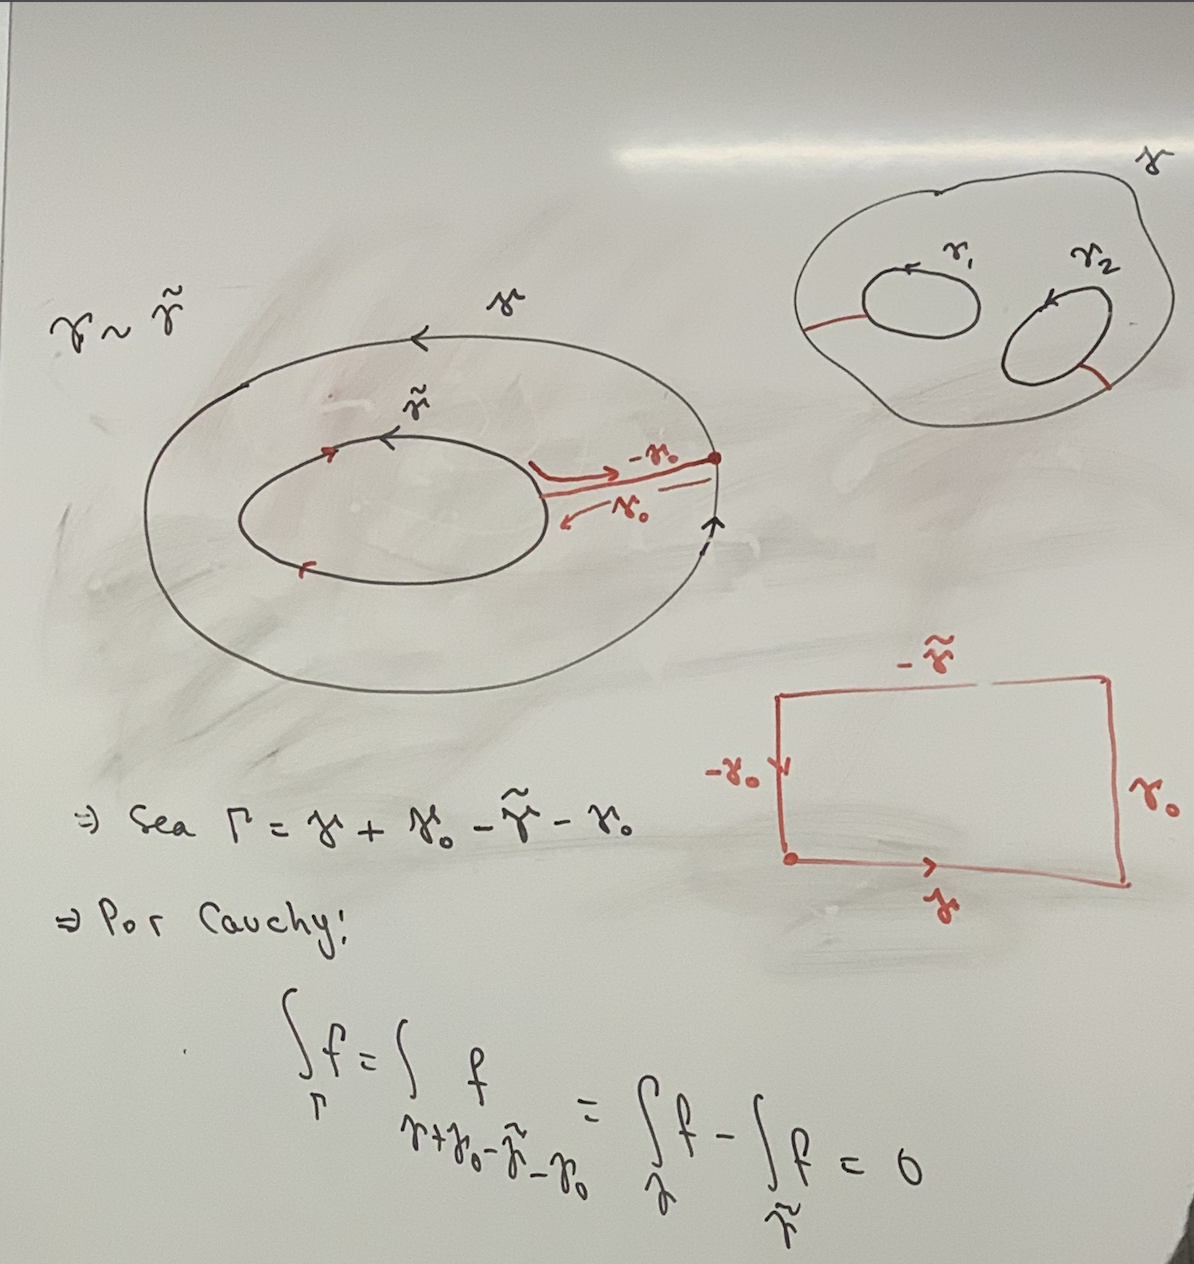
\includegraphics[scale=0.4]{imagenes/11.2}
    \end{figure}
\end{teorema}